\begin{wrapfigure}{r}{0.5\textwidth}
  \centering
  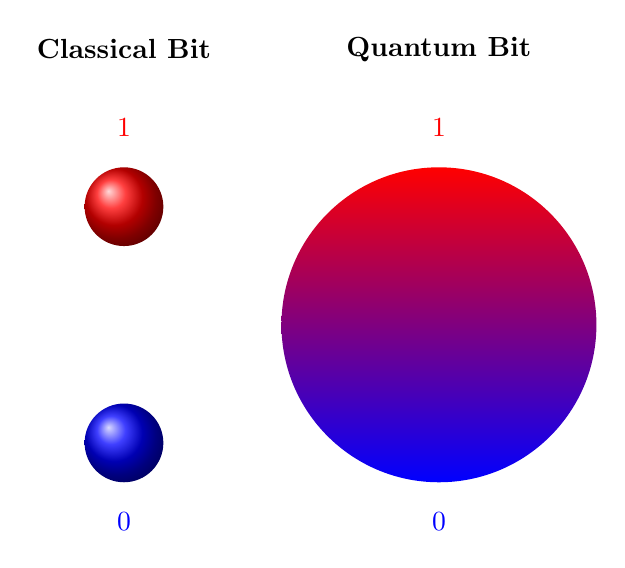
\begin{tikzpicture}[scale=1]
    \node[font=\bfseries] at (0,2) {Classical Bit};
    \node[font=\bfseries] at (4,2) {Quantum Bit};

    \node[color=red] at (0,1) {$1$};
    \node[color=blue] at (0,-4) {$0$};

    \node[shade,shading=ball,circle,ball color=blue,minimum size=1cm] (ball) at (0,-3) {};
    \node[shade,shading=ball,circle,ball color=red,minimum size=1cm] (ball) at (0,0) {};

    \node[color=red] at (4,1) {$1$};
    \node[color=blue] at (4,-4) {$0$};
    \node[shade, shading=ball,circle,top color=red, bottom color=blue, minimum size=4cm] (ball) at (4,-1.5) {};
  \end{tikzpicture}
  \caption{Conceptual illustration of the two-level classical bit, which are restricted to the boolean states 1 (true) or 0 (false), and the quantum bit that can be in any superposition of the states 0 or 1.}
  \label{fig:qubit and bit}
\end{wrapfigure}
